\documentclass{standalone}

\usepackage{tikz}
\usepackage{amssymb}
\usetikzlibrary{calc, positioning}
\begin{document}
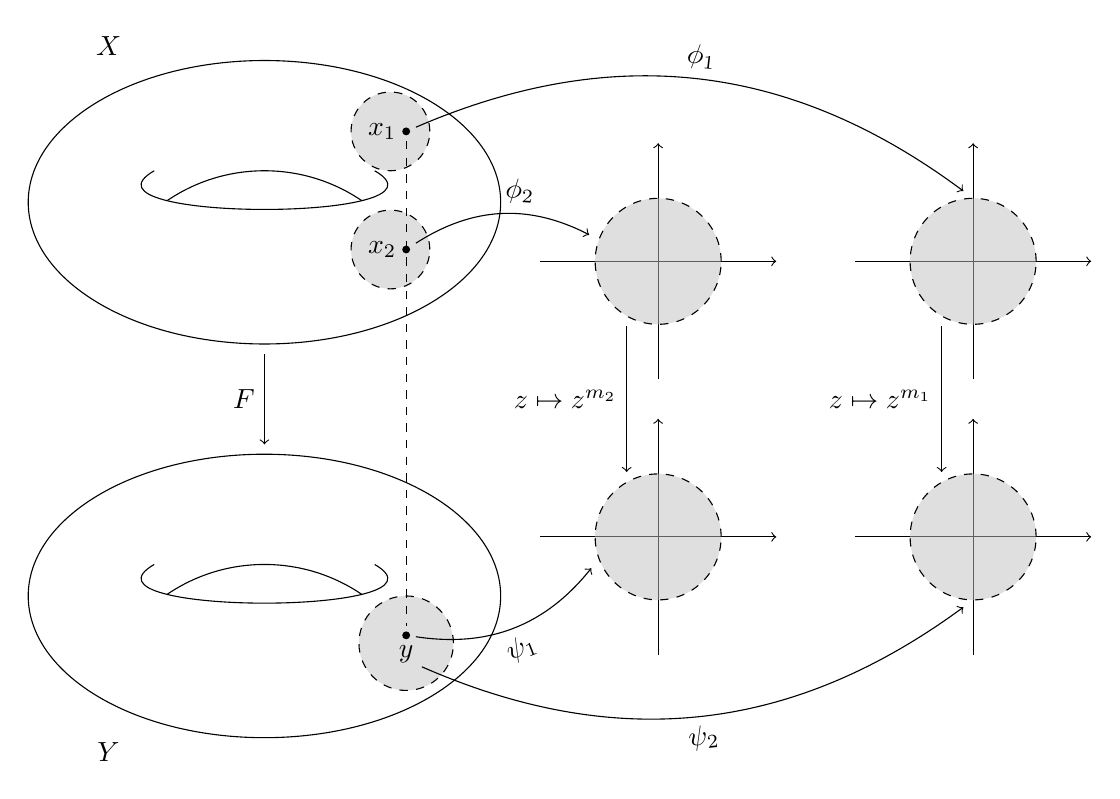
\begin{tikzpicture}
	\begin{scope}
		\node at (135:2.8) {$ X $};
		\draw (0,0) ellipse (3 and 1.8);
		\begin{scope}
			\draw[looseness=1.2] (-1.4,0.4) to[out=210, in=-30] (1.4,0.4);
			\clip[looseness=1.2] (-1.4,0.4) to[out=210, in=-30] (1.4,0.4)
			to cycle;
			\draw (0,-1.8) circle (2.2);
		\end{scope}
		\node (x1) at (1.8,0.9){};
		\node (x2) at (1.8,-0.6){};
		\node (t) at (0,-1.8){};
		\filldraw[fill=gray!50, fill opacity=0.5, dashed] ($ (x1) + (-0.2, 0) $)
		circle (0.5);
		\filldraw[fill=gray!50, fill opacity=0.5, dashed] ($ (x2) + (-0.2, 0) $)
		circle (0.5);
		\fill (x1) circle (0.05) node[left]{$ x_1 $};
		\fill (x2) circle (0.05) node[left]{$ x_2 $};
	\end{scope}

	\begin{scope}[yshift=-5cm]
		\node at (-135:2.8) {$ Y $};
		\draw (0,0) ellipse (3 and 1.8);
		\begin{scope}
			\draw[looseness=1.2] (-1.4,0.4) to[out=210, in=-30] (1.4,0.4);
			\clip[looseness=1.2] (-1.4,0.4) to[out=210, in=-30] (1.4,0.4)
			to cycle;
			\draw (0,-1.8) circle (2.2);
		\end{scope}
		\node (y1) at (1.8,-0.5){};
		\node (b) at (0,1.8){};
		\filldraw[dashed, fill=gray!50, fill opacity=0.5] ($ (y1) - (0,0.1) $) circle (0.6);
		\fill (y1) circle (0.05) node[below]{$ y $};
	\end{scope}

	\begin{scope}[xshift=5cm]
		\begin{scope}[yshift=-0.75cm]
			\draw[->] (-1.5,0) -- (1.5,0);
			\draw[->] (0,-1.5) -- (0,1.5);
			\filldraw[dashed, fill=gray!50, fill opacity = 0.5] (0,0) circle (0.8);
			\node (mtr) at (160:0.8){};
			\node (mf1) at (-0.4, -0.7){};
		\end{scope}

		\begin{scope}[yshift=-4.25cm]
			\draw[->] (-1.5,0) -- (1.5,0);
			\draw[->] (0,-1.5) -- (0,1.5);
			\filldraw[dashed, fill=gray!50, fill opacity = 0.5] (0,0) circle (0.8);
			\node (mbr) at (-160:0.8){};
			\node (mf2) at (-0.4, 0.7){};
		\end{scope}
	\end{scope}

	\begin{scope}[xshift=9cm]
		\begin{scope}[yshift=-0.75cm]
			\draw[->] (-1.5,0) -- (1.5,0);
			\draw[->] (0,-1.5) -- (0,1.5);
			\filldraw[dashed, fill=gray!50, fill opacity = 0.5] (0,0) circle (0.8);
			\node (rtr) at (90:0.8){};
			\node (rf1) at (-0.4, -0.7){};
		\end{scope}

		\begin{scope}[yshift=-4.25cm]
			\draw[->] (-1.5,0) -- (1.5,0);
			\draw[->] (0,-1.5) -- (0,1.5);
			\filldraw[dashed, fill=gray!50, fill opacity = 0.5] (0,0) circle (0.8);
			\node (rbr) at (-90:0.8){};
			\node (rf2) at (-0.4, 0.7){};
		\end{scope}
	\end{scope}

	\draw[dashed] (x1) -- (y1);
	\draw[->] (t) to node[left]{$ F $} (b);
	\draw[->, bend left, sloped] (x2) to node[above, pos=0.6]{$ \phi_2 $} (mtr);
	\draw[->, bend right, sloped] (y1) to node[below]{$ \psi_1 $} (mbr);
	\draw[->, bend left, sloped] (x1) to node[above]{$ \phi_1 $} (rtr);
	\draw[->, bend right, sloped] ($ (y1) + (0.2,-0.4) $) to node[below]{$ \psi_2
		$} (rbr);
	\draw[->] (rf1) to node[left]{$ z \mapsto z ^{m_1} $} (rf2);
	\draw[->] (mf1) to node[left]{$ z \mapsto z ^{m_2} $} (mf2);

\end{tikzpicture}
\end{document}
